\section{Announcements}
\begin{itemize}
    \item Midterm Exam \#3 is Wednesday December 2, from
    \textbf{1:40--3:00 PM}.
    \item Pset \#12: Sampling is due Wednesday December 2 at
    \textbf{11:59 PM}, after the exam.
    \item There is no class on Wednesday November 25 (Thanksgiving week),
    and nothing is due that day.
\end{itemize}

\section{Reminders about sampling of signals}
Use $f$ for frequency in Hz and $\omega=2\pi f$ for angular frequency in rad/s.
For a sampling frequency $F_s$,
\[
T_s=\frac{1}{F_s},\qquad \omega_s=2\pi F_s.
\]
Our continuous-time sampling model and its Fourier transform are
\[
x_s(t)=\sum_{n=-\infty}^{\infty}x(nT_s)\delta(t-nT_s),
\qquad
X_s(\omega)=\frac{1}{T_s}\sum_{k=-\infty}^{\infty}
X(\omega-k\omega_s).
\]
We use the same Fourier transform convention as before:
\[
X(\omega)=\int_{-\infty}^{\infty}x(t)e^{-j\omega t}\,dt,
\qquad
x(t)=\frac{1}{2\pi}\int_{-\infty}^{\infty}X(\omega)e^{j\omega t}\,d\omega.
\]
Two useful tools are
\[
\mathcal{F}\{A\cos(\omega_0t)\}
=A\pi\big[\delta(\omega-\omega_0)+\delta(\omega+\omega_0)\big],
\qquad Y(\omega)=H(\omega)X(\omega).
\]
For a signal with no frequency components above $B$ Hz, use $F_s>2B$
to reconstruct it without aliasing.

\begin{popquiz}
If $F_s=1000$ samples/second, find $T_s$ and $\omega_s$.
If a signal contains frequencies up to 700 Hz, is this sampling rate high
enough to guarantee reconstruction? Explain using both Hz and rad/s.
\popqsplit
We have $T_s=1$ ms and $\omega_s=2000\pi$ rad/s.
A 700 Hz bandwidth requires $F_s>1400$ samples/second, or
$\omega_s>2800\pi$ rad/s, for the sampling-theorem guarantee.
\end{popquiz}

\clearpage

\section*{EE 102: In-class activity on sampling (11/23)}
We have three continuous-time signals: $x_1(t)=\cos(2\pi\,100t)$,  $x_2(t)=\cos(2\pi\,700t)$, $x_3(t)=\cos(2\pi\,950t)$.
We would like to store these signals by taking samples and storing the samples (with the idea that we will be able to reconstruct the signal when needed, using these samples). So, start by calculating some sample values and seeing what they tell us about the signals.

For $x_1(t)$, take samples at
    \(
    t=0,\ 1,\ 2,\ 3,\ 4,\ 5\ \text{ms}
    \)  (don't forget to convert to seconds).
What are the six sample values? What sampling frequency are we using?

Now, let us sample $x_2(t)$ at
    \(
    t=0,\ 3,\ 6,\ 9,\ 12,\ 15\ \text{ms}.
    \)
What are these six sample values? How do they compare with the values you obtained for $x_1(t)$?

You vaguely remember from EE 102 that you have to be careful when taking samples as two very different signals can have the same samples. So, to not make this mistake, you first try to find out whether it is possible to get the same list of sample values from $x_3(t)$.
\begin{enumerate}
    \item What sampling times for $x_3(t)$ will lead to same sample values? 
    \item If we are given the sample values
    and their times, can we tell which of the three signals was sampled?
\end{enumerate}

\textbf{So, how can we sample each of these signals so that we do not lose
any information?} Let us look at the frequency domain for answers:
\begin{enumerate}[label=(\alph*),resume]
    \item Sketch $X_1(\omega)$, $X_2(\omega)$, and
    $X_3(\omega)$.

    \item Write $X_2(\omega)$ in terms of $X_1(\omega)$?
    \item Write $X_3(\omega)$ in terms of $X_1(\omega)$?

    \item Our goal is to recover each original signal from its samples.
    What sampling rate condition do we need for each signal, and what is
    one sampling frequency we can use for each?

\end{enumerate}

Suppose we want one instrument to handle all three signals using the same sampling frequency and the same ideal reconstruction filter. What sampling frequency and filter cutoff can we use? At your new sampling rate, what is each signal's sample value at $t=T_s$?
Do the three signals still give the same value?
\clearpage
\subsection*{Exercise 1: Solution}
For the first signal, the sample spacing is $T_s=1$ ms, so we have
$F_s=1000$ samples/second. Let $t_1=n$ ms, $t_2=3n$ ms, and $t_3=2n$ ms.
The samples at these times are
\begin{center}
\begin{tabular}{c|rrrrrr}
$n$ & 0 & 1 & 2 & 3 & 4 & 5 \\
\hline
$x_1(t_1)$ & 1.000 & 0.809 & 0.309 & $-0.309$ & $-0.809$ & $-1.000$ \\
$x_2(t_2)$ & 1.000 & 0.809 & 0.309 & $-0.309$ & $-0.809$ & $-1.000$ \\
$x_3(t_3)$ & 1.000 & 0.809 & 0.309 & $-0.309$ & $-0.809$ & $-1.000$
\end{tabular}
\end{center}
So, for $x_3(t)$, we can use the times $0,2,4,6,8,10$ ms.
The spacing is 2 ms, giving a sampling frequency of 500 samples/second.
The three signals have the same values at these sampling points:
\[
\begin{aligned}
x_1(n/1000)&=\cos(0.2\pi n),\\
x_2(3n/1000)&=\cos(4.2\pi n)=\cos(0.2\pi n),\\
x_3(2n/1000)&=\cos(3.8\pi n)=\cos(0.2\pi n).
\end{aligned}
\]
This will be impossible to decipher and reconstruct, so we must rethink
our sampling strategy.

Let's see if the frequency domain can help us understand this better.
By taking the Fourier transform of $x_1(t)$, $x_2(t)$, and $x_3(t)$, we get
\[
\begin{aligned}
X_1(\omega)&=\pi\big[\delta(\omega-200\pi)+\delta(\omega+200\pi)\big],\\
X_2(\omega)&=\pi\big[\delta(\omega-1400\pi)+\delta(\omega+1400\pi)\big],\\
X_3(\omega)&=\pi\big[\delta(\omega-1900\pi)+\delta(\omega+1900\pi)\big].
\end{aligned}
\]
For the relationships between the spectra, we have $x_2(t)=x_1(7t)$ and
$x_3(t)=x_1(\frac{19}{2}t)$. Substituting $u=7t$ in the Fourier transform of $x_2(t)$
gives
\[
X_2(\omega)=\frac{1}{7}\int_{-\infty}^{\infty}
x_1(u)e^{-j(\omega/7)u}\,du
=\frac{1}{7}X_1\!\left(\frac{\omega}{7}\right).
\]
Similarly,
\[
X_3(\omega)=\frac{2}{19}X_1\!\left(\frac{2\omega}{19}\right).
\]

The original signals have highest frequencies of 100, 700, and 950 Hz.
To recover each original signal using the sampling theorem, we can choose
the rates as follows:
\begin{center}
\begin{tabular}{c|c|c}
Signal & Sampling-rate condition & One possible rate \\
\hline
$x_1(t)$ & $F_s>200$ & 400 samples/second \\
$x_2(t)$ & $F_s>1400$ & 2000 samples/second \\
$x_3(t)$ & $F_s>1900$ & 2000 samples/second
\end{tabular}
\end{center}
A sampling rate of 1000 samples/second is sufficient for $x_1(t)$, but not for $x_2(t)$ or $x_3(t)$.

For one instrument that can handle all three, we can use
$F_s=2000$ samples/second and an ideal reconstruction filter with a
1000 Hz cutoff and gain $T_s=1/2000$. The highest original frequency is
950 Hz, while the nearest replica begins at $2000-950=1050$ Hz.
Our cutoff lies between them, so we can recover each original signal.
At the first sample after zero, $t=T_s=1/2000$ seconds, we have
\[
\begin{aligned}
x_1(T_s)&=\cos(\pi/10),\\
x_2(T_s)&=\cos(7\pi/10),\\
x_3(T_s)&=\cos(19\pi/20).
\end{aligned}
\]
The three sample values are different. With this sampling and reconstruction
setup, we can recover the original frequency of each signal.


\begin{figure}[htbp]
\centering
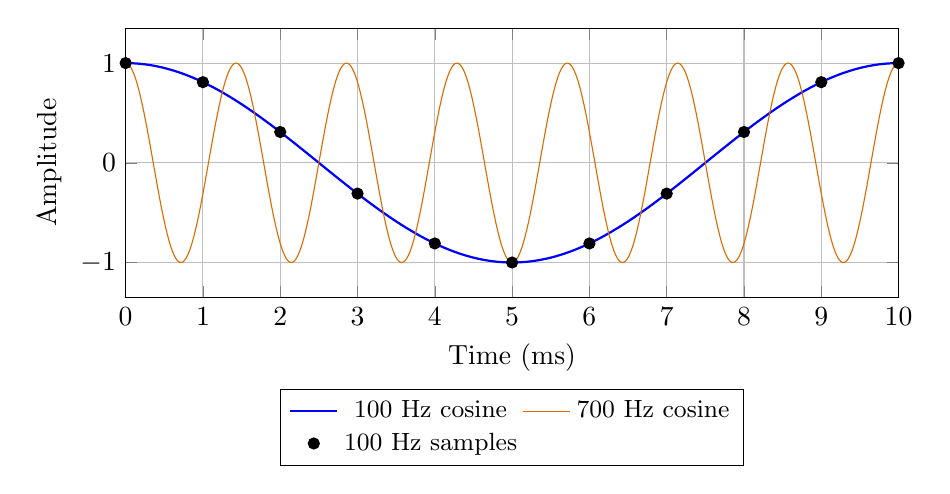
\begin{tikzpicture}
\begin{axis}[
    width=0.94\linewidth,height=5cm,
    xlabel={Time (ms)},ylabel={Amplitude},
    xmin=0,xmax=10,ymin=-1.35,ymax=1.35,
    xtick={0,1,...,10},grid=major,
    legend style={at={(0.5,-0.34)},anchor=north,legend columns=2,font=\small}
]
\addplot[blue,thick,domain=0:10,samples=501] {cos(36*x)};
\addlegendentry{100 Hz cosine}
\addplot[orange!85!black,domain=0:10,samples=901] {cos(252*x)};
\addlegendentry{700 Hz cosine}
\addplot[only marks,black,mark=*,mark size=2pt,domain=0:10,samples=11]
    {cos(36*x)};
\addlegendentry{100 Hz samples}
\end{axis}
\end{tikzpicture}
\caption{The 100 Hz signal sampled every 1 ms and the 700 Hz signal sampled every 3 ms give the same ordered sample values.}
\end{figure}

\clearpage
\section{Practice problem}
\begin{popquiz}
We have a signal
\[
x(t)=A\cos(2\pi\,100t).
\]
Our measurement also contains
\[
v(t)=B\cos(2\pi\,900t),\qquad r(t)=x(t)+v(t).
\]
The amplitudes $A$ and $B$ are unknown. We will sample $r(t)$ at
$F_s=1000$ samples/second. Then, we will pass the sampled signal through
an ideal low-pass reconstruction filter with a cutoff of 500 Hz and
gain $T_s$.
\begin{enumerate}[label=(\alph*)]
    \item What is the reconstructed signal $y(t)$?
    \item Can we design a filter after sampling to keep the desired
    100 Hz component unchanged and remove the interference? What
    information do the samples give us about $A$ and $B$?
    \item Design an ideal low-pass filter to keep $x(t)$ and remove
    $v(t)$ before sampling. Choose your cut-off frequency and gain.
    Sketch the complete sampling and reconstruction process and find
    its output.
    \item If we want to reconstruct the entire signal $r(t)$,
    including its 900 Hz component, what sampling-rate condition do
    we need?
\end{enumerate}
\popqsplit
At $t=n/1000$, the 100 Hz and 900 Hz cosines have the same values, so
\[
r(nT_s)=(A+B)\cos(0.2\pi n).
\]
The reconstructed signal is
\[
y(t)=(A+B)\cos(2\pi\,100t).
\]
The samples determine $A+B$, which does not determine the unknown amplitude
$A$. After sampling, both contributions occupy the same frequency.
A filter cannot pass one of these contributions unchanged and suppress
the other by selecting frequencies.

We can design an ideal low-pass filter with a 200 Hz cutoff and gain 1:
\[
H_A(\omega)=
\begin{cases}
1,& |\omega|<400\pi,\\
0,& |\omega|\geq400\pi.
\end{cases}
\]
It passes 100 Hz and removes 900 Hz before the interference can alias.
Sampling and reconstruction then give
\[
y(t)=A\cos(2\pi\,100t)=x(t).
\]
To reconstruct the entire signal $r(t)$ using the sampling theorem,
we need $F_s>1800$ samples/second and a suitable reconstruction filter.
\end{popquiz}

\begin{figure}[htbp]
\centering
\begin{tikzpicture}[node distance=0.65cm]
\node (input) {$r(t)$};
\node[block,right=of input,minimum width=2.2cm] (analog)
    {Analog LPF\\200 Hz, gain 1};
\node[block,right=of analog,minimum width=2.2cm] (sampler)
    {Sampler\\$F_s=1000$};
\node[block,right=of sampler,minimum width=2.5cm] (recon)
    {Reconstruction\\500 Hz, gain $T_s$};
\node[right=of recon] (output) {$x(t)$};
\draw[conn] (input) -- (analog);
\draw[conn] (analog) -- (sampler);
\draw[conn] (sampler) -- (recon);
\draw[conn] (recon) -- (output);
\end{tikzpicture}
\caption{The low-pass filter removes the unwanted frequency component before
sampling. The reconstruction filter then recovers $x(t)$.}
\end{figure}
